\documentclass[conference]{IEEEtran}
\usepackage{graphicx}
\usepackage{tikz}
\usepackage[colorlinks = true, citecolor = blue]{hyperref}

% math lib
\usepackage{amsmath}
\usepackage{mathrsfs}

% operators
\DeclareMathOperator*{\argmax}{arg\,max}
\DeclareMathOperator*{\argmin}{arg\,min}
\newcommand\ceiling[1]{\left\lceil #1 \right\rceil}

% empty set
\usepackage{amssymb}
\let\emptyset=\varnothing

% algorithms
\usepackage{algorithm}
\usepackage{algorithmic}
\renewcommand{\algorithmicrequire}{\textbf{Input:}}
\renewcommand{\algorithmicensure}{\textbf{Output:}}

\begin{document}
% --------------------------------------------
% --------------Change HERE! -----------------
% --------------------------------------------
\def\authorone{Durga Muralidharan}
\def\authortwo{Devi Surya Kumari Akula}
\def\groupid{3}
% --------------------------------------------
\title{CS258 Final Report: The RSA Problem}
\author{
    \IEEEauthorblockN{\authorone\ and \authortwo}
    \IEEEauthorblockA{
        Group \groupid
    }    
}

\maketitle
\IEEEpeerreviewmaketitle

\section{Methods: RL-based Routing}
\vspace{0.5em}

% List RL algorithms and give a brief explanation of each
\subsection{RL Algorithms}
\vspace{0.5em}

\begin{enumerate}
    \item \textbf{Proximal Policy Optimization (PPO) }\cite{schulman2017proximal}
    is a state-of-the-art policy gradient method used in reinforcement learning, developed by OpenAI. It improves upon traditional policy gradient methods like Trust Region Policy Optimization (TRPO) by using a clipped objective function to ensure more stable and reliable updates. It strikes a balance between exploration and exploitation by limiting the deviation of the new policy from the old policy, thus preventing large, destabilizing policy updates and promoting steady, stable learning. \vspace{0.5em}
    
    \item \textbf{Deep Q-learning (DQN)} \cite{mnih2013playing}
     is a reinforcement learning algorithm that combines Q-learning (a model-free RL algorithm used to find the optimal action-selection policy for a given finite Markov Decision Process) with deep neural networks. It was proposed by researchers at DeepMind to enable RL agents to learn policies directly from high-dimensional sensory inputs, such as raw pixel data in video games. DQN uses a neural network to approximate the Q-value function, which predicts the expected cumulative reward for each action in a given state, and employs experience replay and target networks to stabilize and improve the learning process.
\end{enumerate}

\subsection{State Space}
\vspace{0.5em}
% Explain state/action/reward
% Make sure you provide enough information to reconstruct results
% Check https://gymnasium.farama.org/environments/box2d/lunar_lander/ for some examples
The state space represents the network state and contains the request to be handled, the k-shortest simple paths available between source and destination nodes, and edge statistics. The request includes the source node, destination node, and holding time as a dictionary. Simple paths between a source and destination do not repeat nodes, and we consider the k-shortest paths for this experiment. The paths are expressed as a two-dimensional array of size (k, num\_nodes). Edge statistics contain the available colors for each edge present in the graph. It is a three-dimensional array of size (link\_capacity, num\_nodes, num\_nodes), and each value represents if the color is occupied. A value of -1 represents no edge between the nodes, zero means that the color is available for use, and any value greater than zero represents the time step until which the color is occupied. For example, if the value is 12, the color on that edge is occupied for 12 time steps.

\subsection{Action Space}
\vspace{0.5em}
The action space is a discrete value between 0 and k. It represents the path to be taken for the current request and maps to the k-shortest paths available in the observation space. Each time a new request arrives, the k-shortest paths between the source and destination nodes are updated in the observation space. The agent then chooses one of these paths as the action.

\subsection{Reward Function}
\vspace{0.5em}
The agent receives different rewards based on the action it takes. A non-blocking path between two nodes means that at least one color is available on all the edges between these nodes.
\begin{itemize}
    \item CASE-1: When the agent chooses a non-blocking path and other non-blocking paths exist, it is rewarded +1.
    \item CASE-2: When the agent chooses the only available non-blocking path, it is rewarded +2.
    \item CASE-3: When the agent chooses a blocking path when other non-blocking paths exist between the source and destination nodes, it is penalized with -2.
    \item CASE-4: When no non-blocking path exists between the nodes, the agent receives neither a reward nor a penalty.
    \item CASE-5: If the agent chooses a path that does not exist between the source and destination nodes, it is penalized with a -5 reward. This happens when two nodes have only one path connecting them.
\end{itemize}
 

\section{Method: Spectrum Allocation}
\vspace{0.5em}
% Explain your heuristic
% If you have multiple, you can make subsections 

% If you borrow some ideas from papers, cite them with bibtex (e.g. \cite{8509143})
We employ a greedy strategy to select the spectrum for handling incoming requests. The request is assigned the lowest indexed color available across all links in the chosen path.

\section{Results}
\vspace{0.5em}

\subsection{Learning Curve}
\vspace{0.5em}
For all experiments performed, k is chosen to be 2. The episode vs. reward mean curve obtained from PPO algorithm for the source-destination pair (San Diego Supercomputer Center to Jon Von Neumann Center, Princeton, NJ) is as shown in Figure \ref{fig:case1_ppo}. Although the reward granted initially decreases, the agent learns to make the right choices which results in increasing reward.
\vspace{\baselineskip}
\begin{figure}[h]
    \centering
    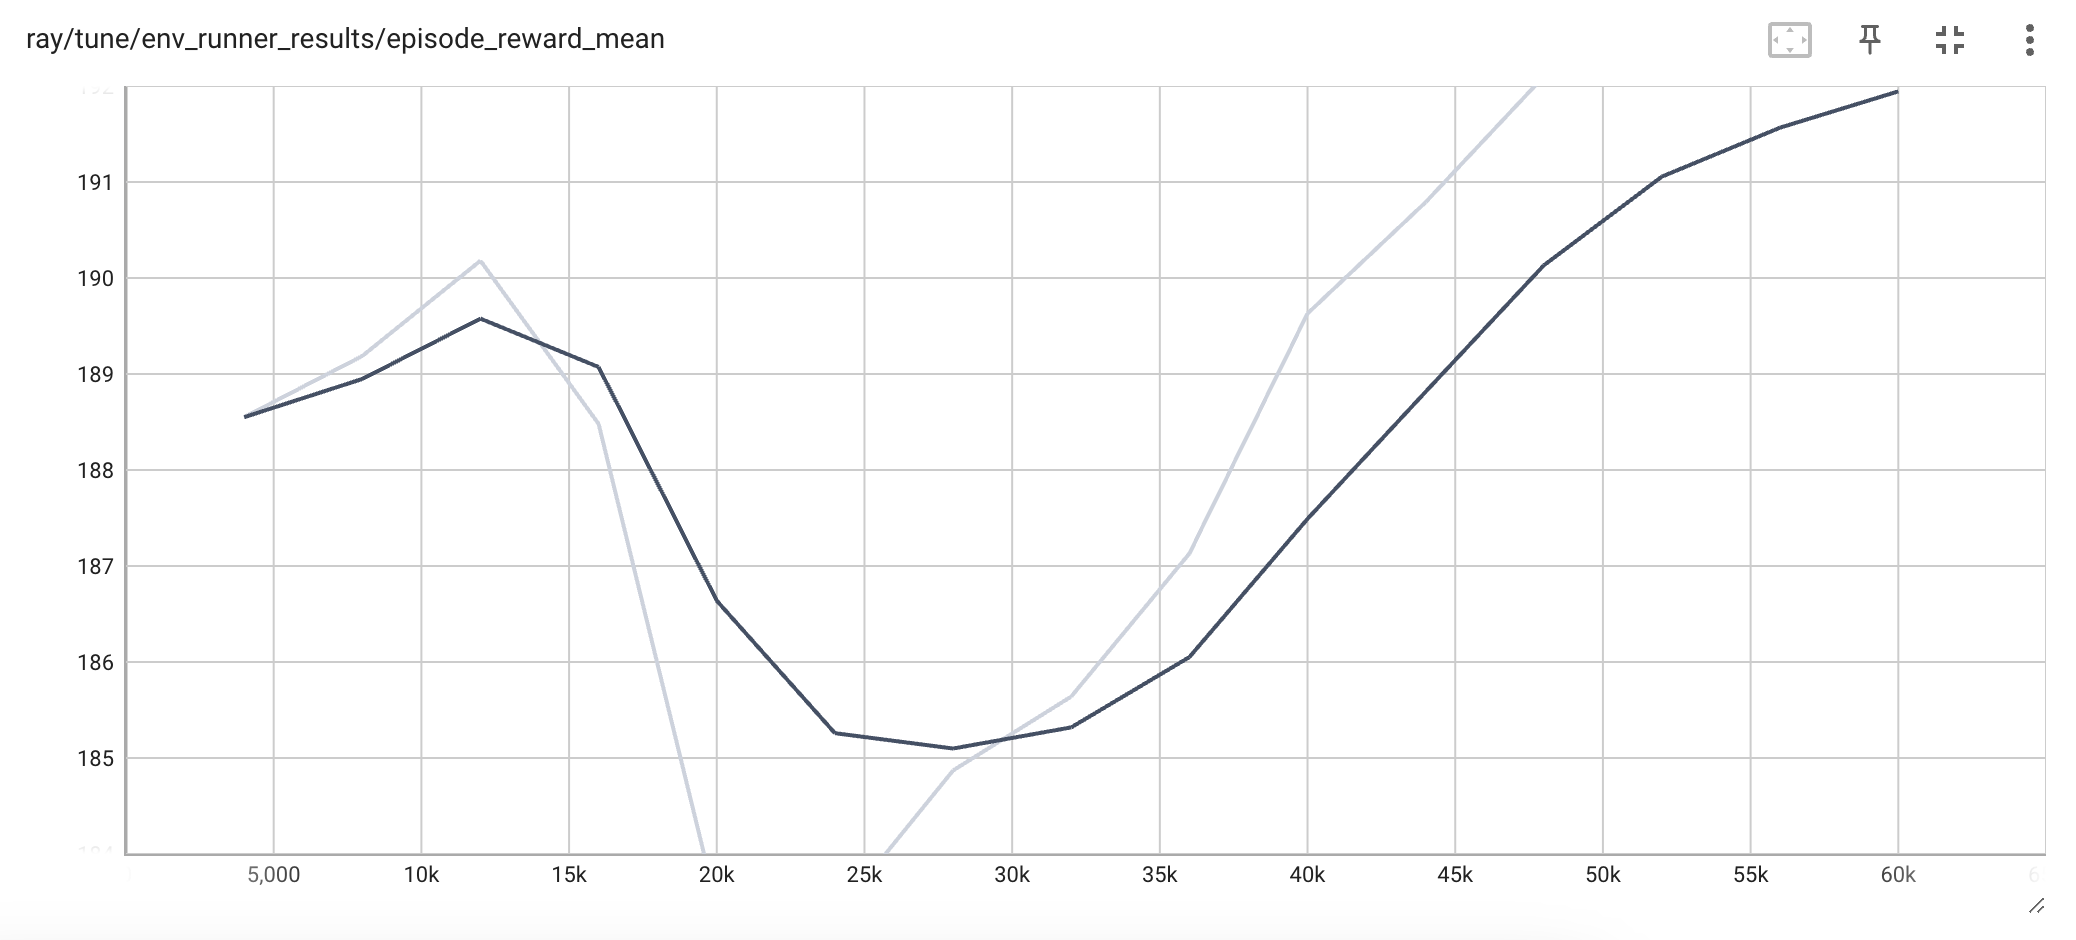
\includegraphics[width=0.4\textwidth]{Figures/case1_ppo.png}
    \caption{Episode vs Reward Mean using PPO for Case1}
    \label{fig:case1_ppo}
\end{figure}

\vspace{0.5em}
Figure \ref{fig:case2_ppo} shows the episode vs. reward mean curve obtained from PPO algorithm for randomly generated source and destination pairs. The agent does not seem to learn as can be seen from the learning curve and the reason could be the randomness of the source and destination nodes. The algorithm learns for fixed source and destination whereas it fails to learn over randomly generated nodes. This could be because, it is unable to generalize the learning/reward obtained from one set of nodes to another.
\vspace{\baselineskip}
\begin{figure}[h]
    \centering
    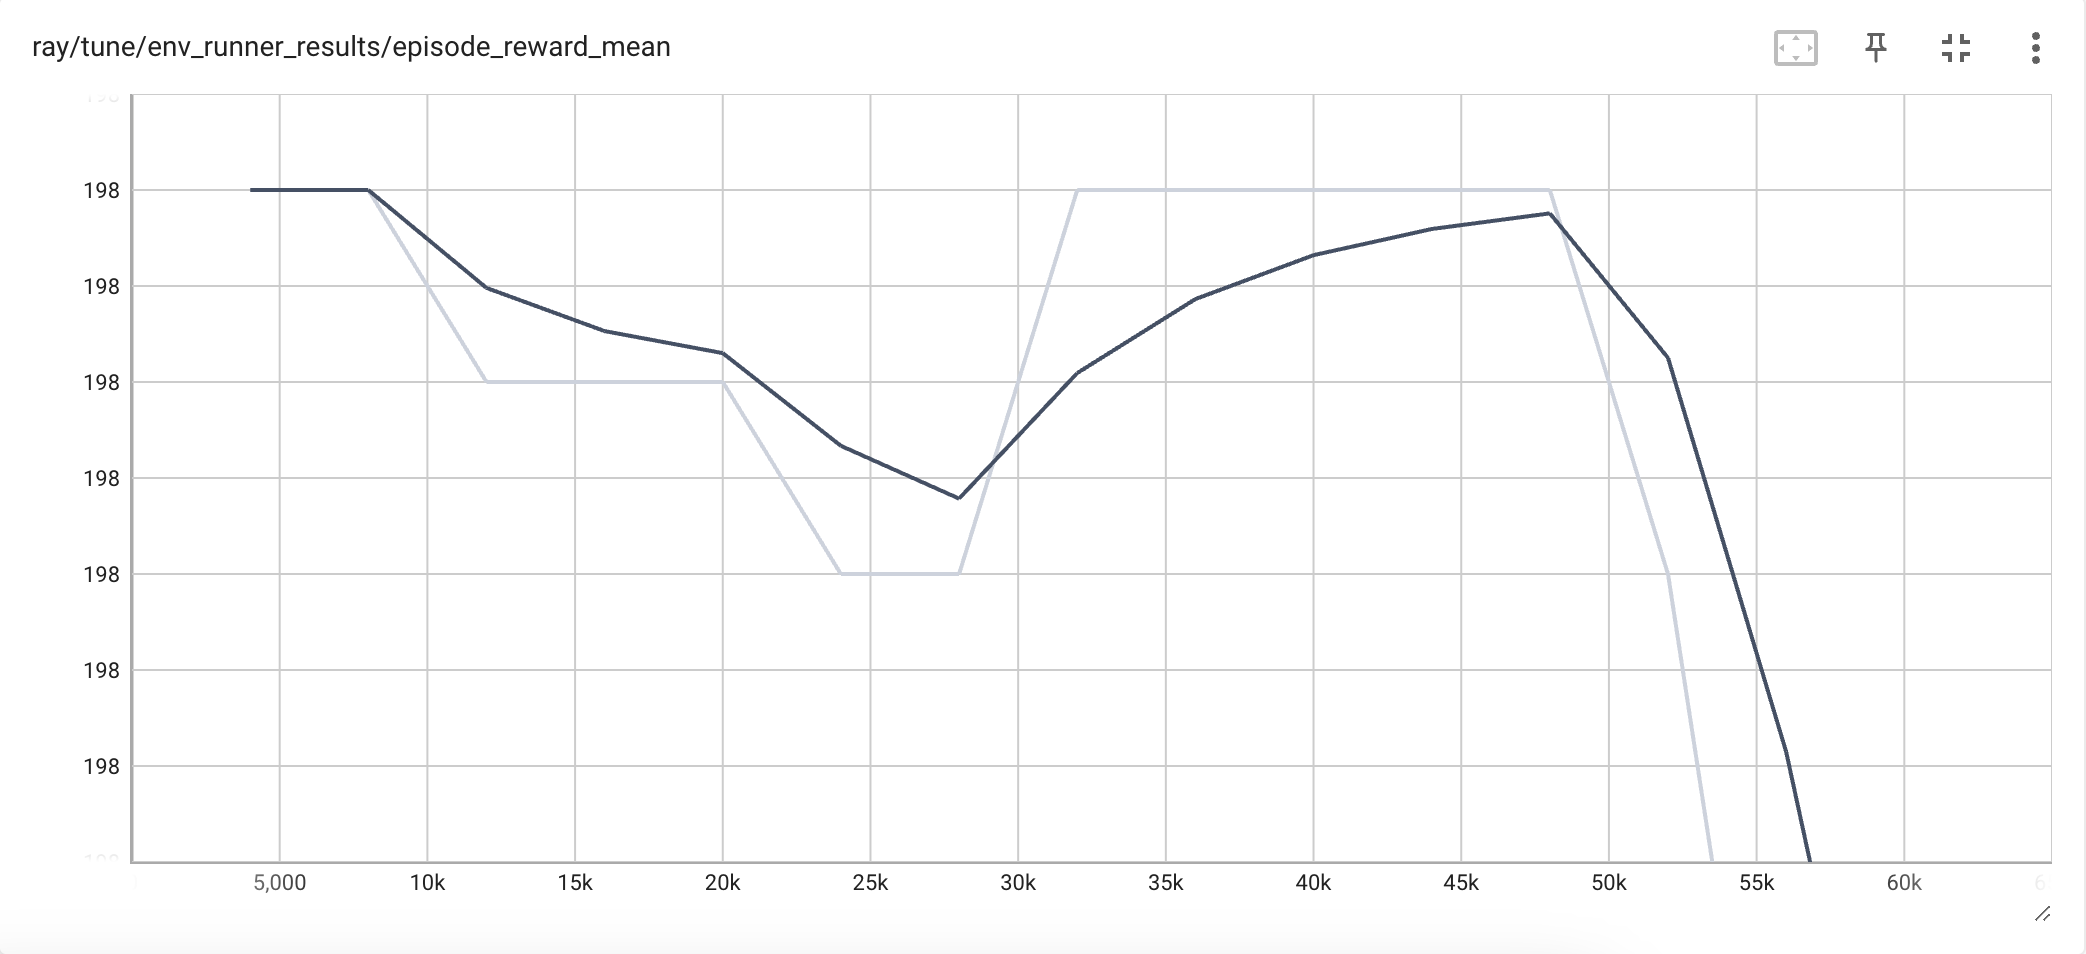
\includegraphics[width=0.4\textwidth]{Figures/case2_ppo.png}
    \caption{Episode vs Reward Mean using PPO for Case2}
    \label{fig:case2_ppo}
\end{figure}

\vspace{0.5em}
The learning curve obtained for fixed source and destination nodes using the DQN algorithm is as shown in Figure \ref{fig:case1_dqn}. It can be seen that the agent learns consistently to increase the reward obtained. On the contrary, it can be seen from Figure \ref{fig:case2_dqn} that the agent does not learn anything when source and destination nodes are generated randomly. Similar to PPO, the reason could be that the DQN algorithm is unable to generalize over random nodes. It may not be able to learn from the updates made to available colors between different edges which is a three-dimensional array in the observation space. This three-dimensional array is also sparse, which could be another reason for the poor learning performance of these algorithms with random node selection.
\vspace{\baselineskip}
\begin{figure}[h]
    \centering
    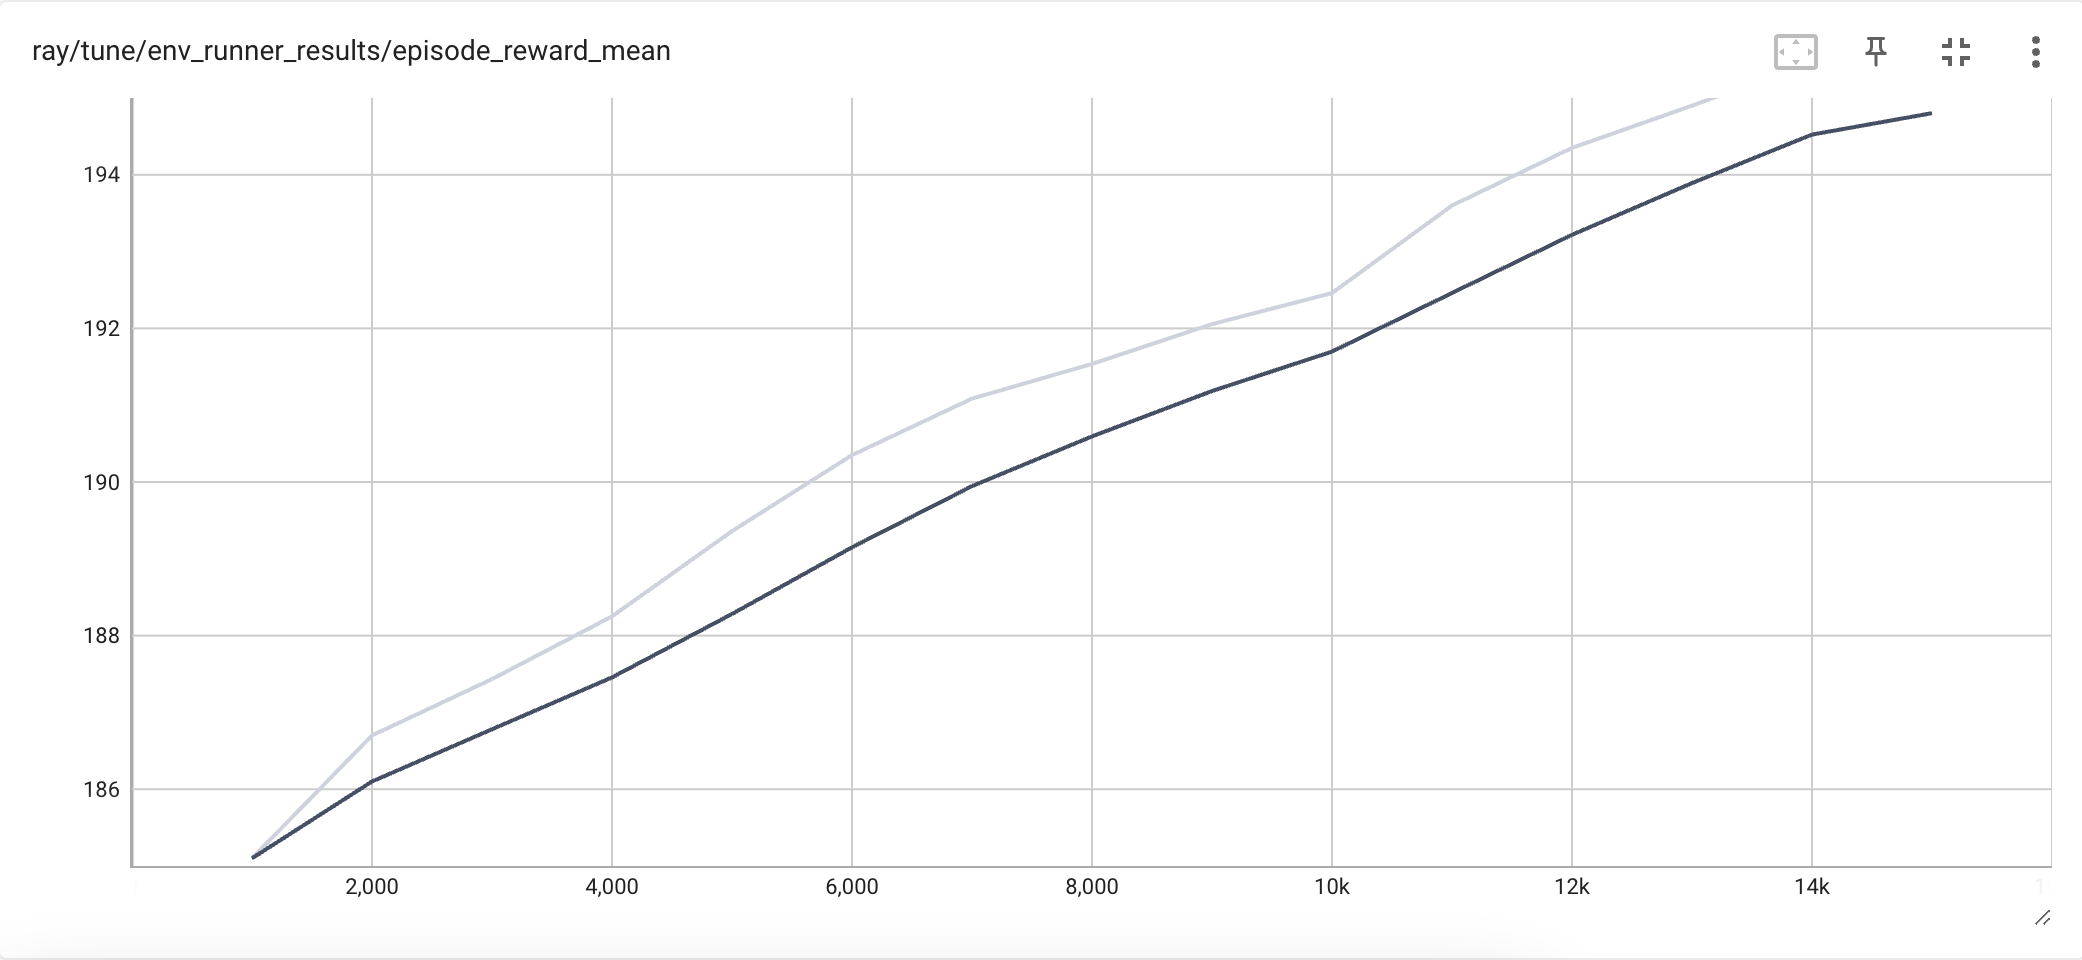
\includegraphics[width=0.4\textwidth]{Figures/case1_dqn.png}
    \caption{Episode vs Reward Mean using DQN for Case1}
    \label{fig:case1_dqn}
\end{figure}

\vspace{\baselineskip}
\begin{figure}[h]
    \centering
    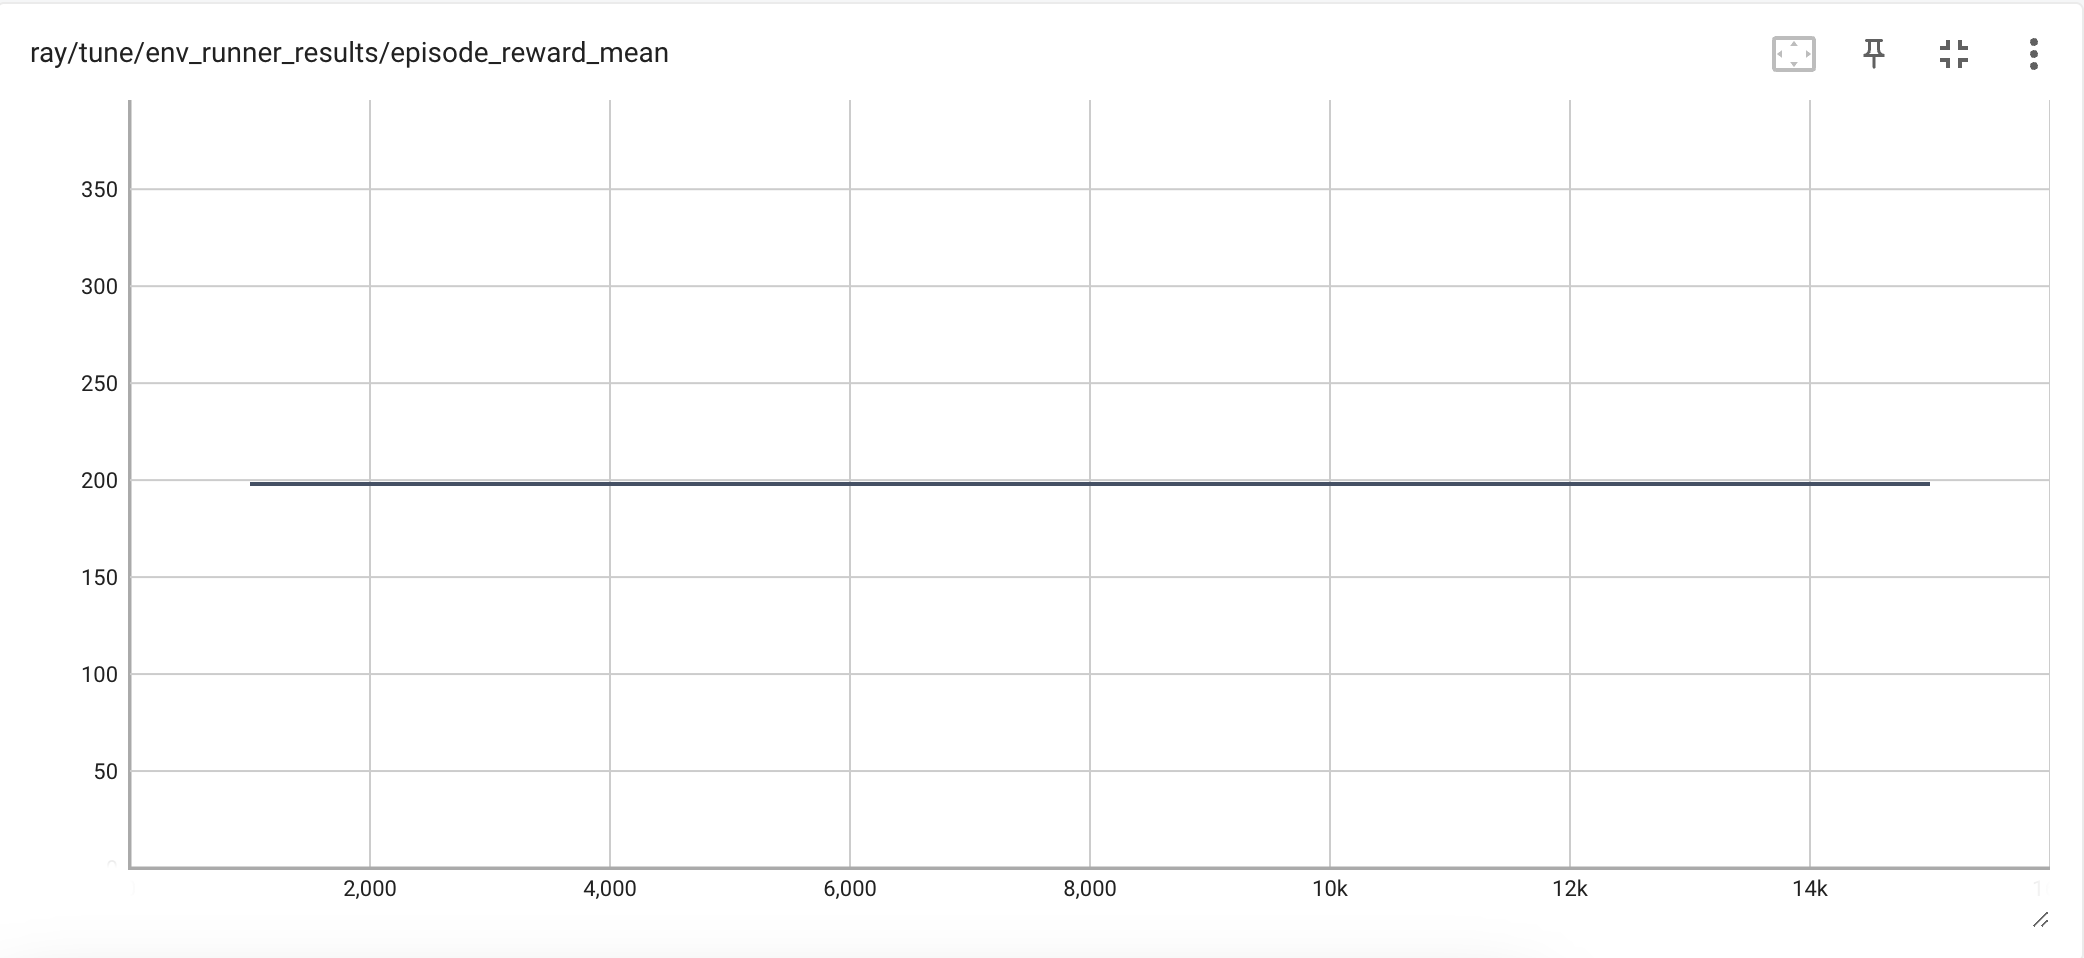
\includegraphics[width=0.4\textwidth]{Figures/case2_dqn.png}
    \caption{Episode vs Reward Mean using DQN for Case2}
    \label{fig:case2_dqn}
\end{figure}
% Insert figures
% Explain the results

\subsection{Utilization (The Objective)}
\vspace{0.5em}
The objective function is calculated as the overall network utilization over all the edges of the graph for every episode. It is calculated after all the 100 requests are handled by the network and the episode is terminated. The objective function does not vary with episode when source and destination nodes are fixed as seen in figures \ref{fig:case1_ppo_obj} and \ref{fig:case1_dqn_obj}. This is because, only a constant number of edges participate and the network utilization remains nearly constant. On the other hand, utilization does not change even when source and destination nodes are randomly generated as in figures \ref{fig:case2_ppo_obj} and \ref{fig:case2_dqn_obj}. This may be due to the network topology that choosing different paths does not affect the overall network utilization. Moreover, the low number of requests being handled, consistently under utilizes the network during every episode and therefore does not vary.
\vspace{\baselineskip}
\begin{figure}[h]
    \centering
    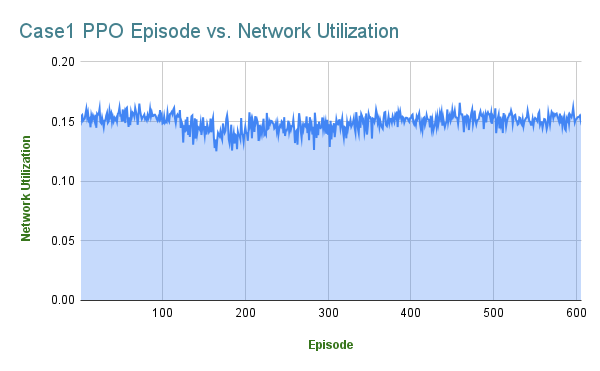
\includegraphics[width=0.4\textwidth]{Figures/Case1 PPO Episode vs. Network Utilization.png}
    \caption{Episode vs Objective Function using PPO for Case1}
    \label{fig:case1_ppo_obj}
\end{figure}

\vspace{\baselineskip}
\begin{figure}[h]
    \centering
    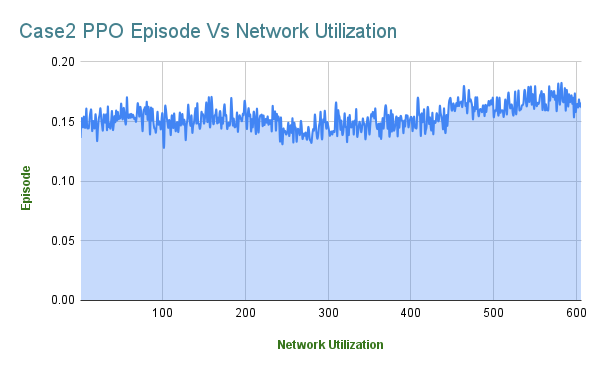
\includegraphics[width=0.4\textwidth]{Figures/Case2 PPO Episode Vs Network Utilization.png}
    \caption{Episode vs Objective Function using PPO for Case2}
    \label{fig:case2_ppo_obj}
\end{figure}

\vspace{\baselineskip}
\begin{figure}[h]
    \centering
    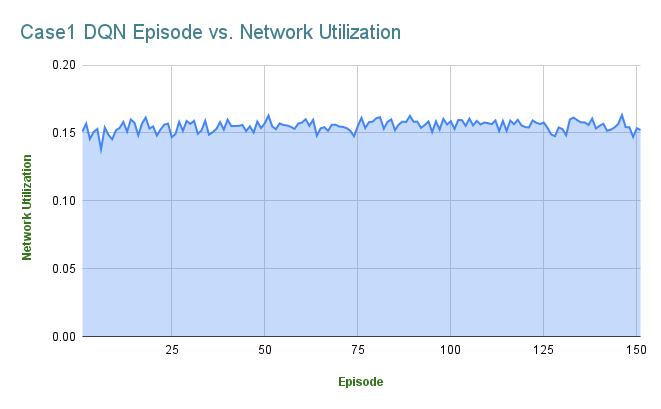
\includegraphics[width=0.3\textwidth]{Figures/Case1 DQN Episode vs. Network Utilization.png}
    \caption{Episode vs Objective Function using DQN for Case1}
    \label{fig:case1_dqn_obj}
\end{figure}

\vspace{\baselineskip}
\begin{figure}[h]
    \centering
    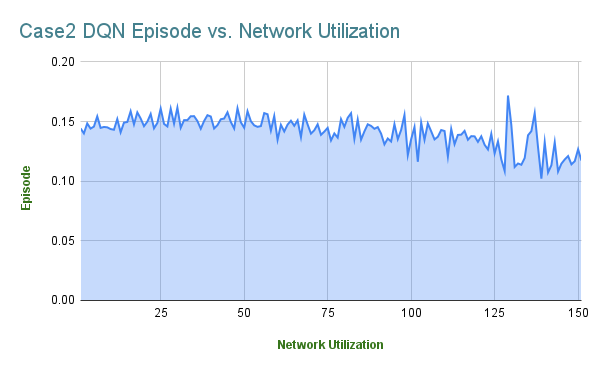
\includegraphics[width=0.3\textwidth]{Figures/Case2 DQN Episode vs. Network Utilization.png}
    \caption{Episode vs Objective Function using DQN for Case2}
    \label{fig:case2_dqn_obj}
\end{figure}

\subsection{Comparison}
\vspace{0.5em}
For the same experiment setup, we can see that DQN performs slightly better than PPO in terms of cumulative reward. DQN has a reward mean of 194 which is slightly higher than the reward mean of 192 obtained by PPO for fixed source and destination. And both algorithms obtain similar network utilization as discussed above.

\vspace{0.5em}
Both algorithms perform slightly better when compared to the network utilization obtained by the simple heuristics. This approach obtains an overall network utilization of 0.0929 when source and destination nodes are fixed and a utilization of 0.109 when random nodes are selected. As can be seen from the figures \ref{fig:case1_ppo_obj},  \ref{fig:case1_dqn_obj}, \ref{fig:case2_ppo_obj}, and \ref{fig:case2_dqn_obj} the network utilization obtained by both RL algorithms is 0.15 on an average.

\bibliography{ref}
\bibliographystyle{ieeetr}


\end{document}